%%
% Modificación de una plantilla de Latex para adaptarla al castellano.
%%

%%%%%%%%%%%%%%%%%%%%%
% Thin Sectioned Essay
% LaTeX Template
% Version 1.0 (3/8/13)
%
% This template has been downloaded from:
% http://www.LaTeXTemplates.com
%
% Original Author:
% Nicolas Diaz (nsdiaz@uc.cl) with extensive modifications by:
% Vel (vel@latextemplates.com)
%
% License:
% CC BY-NC-SA 3.0 (http://creativecommons.org/licenses/by-nc-sa/3.0/)
%
%%%%%%%%%%%%%%%%%%%%%

%----------------------------------------------------------------------------------------
%	PACKAGES AND OTHER DOCUMENT CONFIGURATIONS
%----------------------------------------------------------------------------------------

\documentclass[a4paper, 11pt]{article} % Font size (can be 10pt, 11pt or 12pt) and paper size (remove a4paper for US letter paper)

\usepackage[protrusion=true,expansion=true]{microtype} % Better typography
\usepackage{graphicx} % Required for including pictures
\usepackage[usenames,dvipsnames]{color} % Coloring code
\usepackage{wrapfig} % Allows in-line images
\usepackage[utf8]{inputenc}
\usepackage{enumerate}
\usepackage{enumitem}

% Imágenes
\usepackage{graphicx} 

\usepackage{amsmath}
% para importar svg
%\usepackage[generate=all]{svgfig}

% sudo apt-get install texlive-lang-spanish
\usepackage[spanish]{babel} % English language/hyphenation
\selectlanguage{spanish}
% Hay que pelearse con babel-spanish para el alineamiento del punto decimal
\decimalpoint
\usepackage{dcolumn}
\newcolumntype{d}[1]{D{.}{\esperiod}{#1}}
\makeatletter
\addto\shorthandsspanish{\let\esperiod\es@period@code}
\makeatother

\usepackage{longtable}
\usepackage{tabu}
\usepackage{supertabular}

\usepackage{multicol}
\newsavebox\ltmcbox

% Para algoritmos
\usepackage{algorithm}
\usepackage{algorithmic}
\usepackage{amsthm}

% Para matrices
\usepackage{amsmath}

% Símbolos matemáticos
\usepackage{amssymb}
\usepackage{accents}
\let\oldemptyset\emptyset
\let\emptyset\varnothing

\usepackage[hidelinks]{hyperref}

\usepackage[section]{placeins} % Para gráficas en su sección.
\usepackage[T1]{fontenc} % Required for accented characters
\newenvironment{allintypewriter}{\ttfamily}{\par}
\setlength{\parindent}{0pt}
\parskip=8pt
\linespread{1.05} % Change line spacing here, Palatino benefits from a slight increase by default

\makeatletter
\renewcommand\@biblabel[1]{\textbf{#1.}} % Change the square brackets for each bibliography item from '[1]' to '1.'
\renewcommand{\@listI}{\itemsep=0pt} % Reduce the space between items in the itemize and enumerate environments and the bibliography
\newcommand{\imagen}[2]{\begin{center} \includegraphics[width=90mm]{#1} \\#2 \end{center}}
\newcommand{\RFC}[1]{\href{https://www.ietf.org/rfc/rfc#1.txt}{RFC-#1}}

\renewcommand{\maketitle}{ % Customize the title - do not edit title and author name here, see the TITLE block below
\begin{center} % Center align
{\Huge\@title} % Increase the font size of the title
\end{center}

\vspace{20pt} % Some vertical space between the title and author name

\begin{flushright} % Right align
{\large\@author} % Author name
\\\@date % Date

\vspace{40pt} % Some vertical space between the author block and abstract
\end{flushright}
}
%----------------------------------------------------------------------------------------
%	TITLE
%----------------------------------------------------------------------------------------

\title{\textbf{Protocolos Multimedia}\\ % Title
\vspace{20 pt}
SIP y VoIP} % Subtitle

\author{\textsc{Óscar Bermúdez, Lothar Soto} % Author
\\{\textit{Universidad de Granada}}} % Institution

\date{\today} % Date

%----------------------------------------------------------------------------------------

\begin{document}

\maketitle % Print the title section

{\parskip=2pt
\tableofcontents
}
\pagebreak

\section{SIP}
	\subsection{Historia}
	SIP o Protocolo de Inicio de Sesiones es un protocolo desarrollado por el \textbf{IETF MMUSIC Working Group} con la intención de ser el estándar para la iniciación, modificación y finalización de sesiones interactivas de usuario donde intervienen elementos multimedia.
	
	Puede funcionar en Transmission Control Protocol(\textbf{TCP}), User Datagram Protocol(\textbf{UDP}) o Stream Control Transmission Protocol(\textbf{SCTP}).
	
	Fue publicado en febrero del 1996 en la \RFC{2543}, posteriormente se fueron realizando cambios significativos y se presentó otra versión que se presento como un borrador internacional en 1998. El protocolo consiguió el estatus de Proyecto de Norma en 1999 y la \textbf{IETF} asignó un grupo de trabajo, de manera que podían conocer el crecimiento de dicho protocolo.
	
	En el año 2000 fue proporcionado un borrador que contenía corrección de errores y aclaraciones para SIP publicado en \RFC{2543}. Este documento fue publicado como \RFC{3261} que reemplazó a \RFC{2543}.
	
	\subsection{Funcionalidades SIP}
		\subsubsection{Establecimiento, Modificación y fin de sesión}
		El estandar SIP define la forma en la que se lleva a cabo el establecimiento, modificación y el fin de comunicación multimedia. Usado frecuentemente para añadir nuevos usuarios a una sesión previamente establecida. Para iniciar un proceso de comunicación es necesario que:
		\begin{itemize}
			\item El usuario añadido al proceso debe aceptar participar en dicha sesión.
			\item Los usuarios deben establecer los parámetros multimedia a utilizar.
		\end{itemize}
		El funcionamiento de SIP se realiza de la siguiente forma:
		\begin{itemize}
			\item Los usuarios establecen los códec de voz y video a usar u otros parámetros multimedia.
			\item Si se producen cambios durante la comunicación se notifican a los usuarios que formen parte de la misma.
			\item Por último, en el momento en el que uno de los usuarios desea llevar a cabo la desconexión, se notifica al resto de usuarios de la misma.
		\end{itemize}				
		
		\subsubsection{Movilidad}
		Una de las más importantes ventajas de la telefonía IP es que se puede usar el servicio sin necesidad de encontrarse en una red específica. El protocolo SIP, antes de realizar la comunicación entre usuarios, requiere del reconocimiento de la dirección IP que poseen los participantes además hace uso de las siguientes herramientas:
		\begin{description}
			\item[-]\textbf{URL SIP:} Se le asigna una URL a cada usuario de la red con el objetivo de dar una referencia única en internet. Esta está formada por diferentes campos de información y sigue el siguiente formato:\\
			\textbf{SIP:// <user>: <password> @ <host><tlf>:<PORT>}\\
			El campo de <password> es necesario para la autentificación, si este falta genera un error.
			\item[-]\textbf{Registros:} Esto permite al usuario cambiar su ubicación en lo que a dirección IP se refiere. Al iniciar sesión, se envía un mensaje SIP al servidor donde se especifica el nombre de usuario y la nueva IP asociada a él. Después de esto, si se quiere entablar una comunicación con este usuario, el primer mensaje será dirigido al servidor y la respuesta puede ser dada por un proxy o bién producirse una redirección donde la respuesta será la ubicación de destinatario.
		\end{description}
	
	\subsection{Arquitectura del SIP}
	SIP es un protocolo basado en texto con sintáxis similar al \textbf{HTTP}. Por tanto, tiene 2 tipos de mensajes: \textbf{Peticiones} y \textbf{Respuestas}.
		
		\subsubsection{Peticiones}
		La primera línea de una petición tiene un método y una \textbf{URI} para hacer la petición. Para peticiones SIP, \RFC{3261} definió los siguientes métodos:
		\begin{itemize}
			\item \textbf{REGISTER}: Usado por un agente de usuario para registrarse.
			\item \textbf{INVITE}: Usado para establecer una sesión multimedia entre agentes de usuario.
			\item \textbf{ACK}: Confirma que los intercambios de mensajes son confiables.
			\item \textbf{CANCEL}: Cancela una petición pendiente.
			\item \textbf{BYE}: Termina una sesión.
			\item \textbf{OPTIONS}: Solicita información sobre las posibilidades de un agente de usuario sin la necesidad de comenzar una sesión.
		\end{itemize}
		Más tarde, se introdujeron nuevos métodos en SIP:
		\begin{itemize}
			\item \textbf{PRACK} en el \RFC{3262}.
			\item \textbf{UPDATE} en el \RFC{3311}.
			\item \textbf{MESSAGE} en el \RFC{3428}.
			\item \textbf{REFER} en el \RFC{3515}.
			\item \textbf{PUBLISH} en el \RFC{3903}.
			\item \textbf{INFO} en el \RFC{6086}.
			\item \textbf{NOTIFY} y \textbf{SUBSCRIBE} en el \RFC{6665}.
		\end{itemize}
		
		\subsubsection{Respuestas}
		La primera línea de una respuesta tiene un código de respuesta. Los tipos de respuestas de SIP se clasifican en:
		\begin{itemize}
			\item \textbf{Provisional(1xx)}: La petición fue recibida y está siendo  procesada.
			\item \textbf{Success(2xx)}: La acción fue recibida satisfactoriamente, entendida y aceptada.
			\item \textbf{Redirection(3xx)}: Nuevas acciones necesitan ser realizadas para completar la petición.
			\item \textbf{Client Error(4xx)}: La petición tiene un fallo de sintaxis o no puede ser rellenada por el servidor.
			\item \textbf{Server Error(5xx)}: El servidor falló al rellenar una petición aparentemente válida.
			\item \textbf{Global Failure(6xx)}: La petición no puede ser rellenada en ningún servidor.
		\end{itemize}
	
	\subsection{Servidor SIP}
		En primer lugar un agente de usuario es una entidad de SIP que interactua con el participante de la sesión que tiene normalmente una interfaz para usuario. Son aplicaciones que envian y reciben peticiones SIP.\\
		El servidor SIP acepta las peticiones SIP que se realizan para dar una repsuesta. Un servidor SIP se encarga de llevar a cabo funciones que pueden necesitar los distintos agentes de usuario, este actua en respuesta a una petición de uno de los agentes de usuario.
		
		\subsubsection{Proxy SIP}
			Un servidor Proxy SIP se encarga de recibir peticiones SIP desde un agente de usuario y actuar en nombre de este para la transmision o respuesta a las peticiones.
		
		\begin{figure*}[tbph]
			\centering
			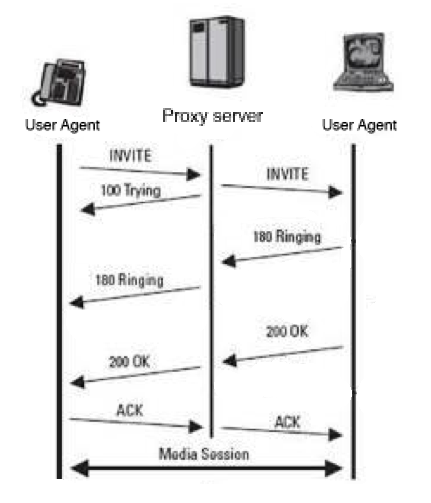
\includegraphics[width=0.7\linewidth]{./Sproxy}
			\caption{Funcionamiento de un servidor proxy}
			\label{fig:Sproxy}
		\end{figure*}
		
		\subsubsection{Servidor de Localización}
			Se encarga de proporcionar información acerca de la localización del usuario. Es necesario conocer el lugar de localización de los usuarios para que la petición de establecimiento de sesión pueda llevarse a cabo.
		
		\subsubsection{Servidor de redireccionamiento SIP}
			Se encarga de aceptar las peticiones SIP y mapea la direccion en nuevas direcciones que son retornadas a los clientes. Estos servidores de redireccionamiento se diferencian  de los servidores proxy en que estos no realizan su propia petición SIP.
	
	\subsection{Aplicaciones del SIP}
		SIP define una arquitectura de señalización y control ampliamente para llamadas de voz y vídeo sobre Internet Protocol(VoIP). También puede ser usado para crear, modificar y terminar sesiones de streaming.
		
		\textbf{OpenWengo}, software libre de telefonía, y \textbf{Gizmo Project}, en software propietario, han implementado SIP en sus clientes y servicios. Ambos programas usan SIP para aceptar las llamadas de un cliente a otro.
		
		Un protocolo de mensajería instantánea basado en SIP, llamado \textbf{SIMPLE}, fue propuesto como estándar y está en desarrollo. \textbf{SIMPLE} puede encargarse de la información de presencia(conocida como el estado en otros clientes de mensajería instantánea), transmitiendo la voluntad de una persona de entablar comunicación con otras.
		
		Otros programas que usan SIP son:
		\textbf{\begin{itemize}
			%\item Jitsi
			%\item Ekiga
			\item Twinkle
			\item Tapioca
			%\item SipX
			%\item KPhone
			\item KCall
			%\item WxCommunicator
			%\item Linphone
			%\item Xlite
			%\item Zoiper
			%\item SJPhone
		\end{itemize}}

\section{VoIP}
	La tecnología VoIP, Voice Over Internet Protocol usa de redes \textbf{IP} y sus protocolos de comunicación de voz, permiten que la voz al igual que los datos utilicen el mismo medio de transmisión. Puede usarse para transportar la comunicación entre dos extremos sea con motivos empresariales o domésticos. También varían los mecanismos de control para garantizar la máxima calidad de servicio.
	
	Existen dos modos de transporte de la voz sobre IP:
		\begin{itemize}
			\item A través de líneas privadas y dedicadas que proporcionan una buena calidad de servicio.
			\item A través de redes públicas como internet, que tienen una calidad de servicio más reducida.
		\end{itemize}
	
	\subsection{Telefonía IP vs. Telefonía Convencional}
		Los sistemas de telefonía tradicional están guiados por un sistema muy simple pero ineficiente denominado conmutación de circuitos.\\
		Para establecer una llamada VoIP, las dos personas deben tener sus teléfonos analógicos conectados a través de un adaptador digital-analógico(\textbf{ATA}).\\
		\begin{tabular}{|p{6cm}|p{6cm}|}
			\hline
			Telefonía convencional & VoIP \\
			\hline \hline
			Se levanta el teléfono y se conecta con el operador local de telefonía. & Se levanta el teléfono, lo que envía una señal al \textbf{ATA}, y éste envía un tono de llamado. \\
			\hline
			Se marca el número de teléfono. & Se marca el número de teléfono. \\
			\hline
			La llamada es transmitida a través del conmutador(\textbf{switch}) de su operador apuntando hacia el teléfono marcado. & Los datos del número son enviados al proveedor de VoIP para revisar que está en un formato válido. \\
			\hline
			Una conexión es creada entre tu teléfono y el de la persona que estás llamando, entremedio el operador comunica las líneas. & El proveedor determina a quién corresponde este número y lo transforma en una dirección \textbf{IP}. \\
			\hline
			El teléfono suena y alguien contesta la llamada. & El proveedor conecta los dos dispositivos que intervienen en la llamada y se envía una señal al \textbf{ATA} del receptor para que suene su teléfono. \\
			\hline
			La conexión abre el circuito. & Cuando alguien contesta, se establece una comunicación tu ordenador y el de la otra persona. La infraestructura de internet maneja los paquetes de voz como haría con un email o con una página web. \\
			\hline
			Uno habla por un tiempo determinado y luego cuelga el teléfono. & Se habla por un periodo de tiempo. Durante la conversación, tu sistema y el del receptor transmiten y reciben paquetes entre sí. \\
			\hline
			Cuando se cuelga el teléfono el circuito automáticamente es cerrado, de esta manera se liberan todas las líneas que intervinieron. & Cuando se termina la llamada, se cuelga el teléfono. En este momento el circuito es cerrado y el \textbf{ATA} envía una señal al proveedor de Telefonía \textbf{IP} informando que la llamada terminó. \\
			\hline
		\end{tabular}
		\label{tabla:vs}
		
		\subsection{Calidad de servicio (QoS)}
		Para poder implementar VoIP(así como otros servicios interactivos), resulta un requisito indespensable la aplicación de QoS.
		
		QoS es el rendimiento promedio visto por los usuarios de una red de telefonía o de ordenadores. Cuantitativamente, se mide considerados varios aspectos del servicio de red:
		\begin{itemize}
			\item Tasas de errores.
			\item Ancho de banda.
			\item Rendimiento.
			\item Retraso en la transmisión.
			\item Disponibilidad.
			\item Jitter(\ref{jitter}).
			\item Y muchos más.
		\end{itemize}
		
		Mucha tecnología ha sido desarrollada para permitir a las redes de ordenadores ser tan útiles como las redes de teléfono para conversaciones de audio, así como el soporte de nuevas aplicaciones con demanda de servicios más estrictos.
		
		Ejemplos de mecanismos de QoS:
		\begin{itemize}
			\item Priorización de tráfico.
			\item Garantía de un ancho de banda mínimo.
		\end{itemize}
	
	\subsection{Requisitos de QoS}
	Se deben tener encuenta que los siguientes ascpectos para garantizar la calidad del sistema:
		
		\subsubsection{Retardo o latencia}
		Establecidos los retardos de tránsito y de procesado de la conversación, la conversación es aceptable si este se encuentra por entre los 50 - 150 ms. 
		El ratardo puede causar dos problemas principales:
		\begin{itemize}
			\item \textbf{Eco}: causado por las señales que se reflejan en el equipo telefónico del extremo opuesto y regresan al hablante.
			\item \textbf{Pérdida de tramas}: se puede ocasionar por una congestión de red o corrupción de datos. Como la voz se transmite a tiempo real, no es práctico retransmitir las tramas perdidas ya que puede producir retardos adicionales. La retransmisión de muestras de voz perdidas son llamadas \textbf{Frame Erasures}. La pérdida de tramas afecta a la calidad de voz dependiendo del modo de gestión de los Frame Erasures que usen los terminales de voz.
		\end{itemize}
		
		\subsubsection{Jitter} \label{jitter}
			Variación de tiempo entre los paquetes causada por la red. Suele considerarse como una señal de ruido, en general como un cambio indeseado y abrupto de la propiedad de una señal. Puede afectar tanto a la amplitud como a la frecuencia o fase.
			Existen distintos tipos:
			\begin{description}
				\item[- Jitter determinista:] Las partes periodicas del jitter. Surge normalmente a partir de señales de ruido externas que se acoplan al sistema de transmisión o las partes del jitter dependientes de los datos. Estas partes dependen de las consecuencias de los datos enviados y son provocadas por la interferencia entre símbolos.
				\item[- Jitter aleatorio:] Este surge a raiz del ruido.
			\end{description}
\end{document}
